\documentclass[11pt,a4paper]{article}
\usepackage{times,latexsym}
\usepackage{url}
\usepackage[T1]{fontenc}


\usepackage{fullpage}


\newcommand\BibTeX{B{\sc ib}\TeX}
\newcommand\confname{EMNLP-IJCNLP 2019}
\newcommand\conforg{SIGDAT}


\usepackage{amsmath}
\usepackage{tikz-dependency}
\DeclareMathOperator*{\argmax}{arg\,max}
\DeclareMathOperator*{\argmin}{arg\,min}
\DeclareMathOperator{\E}{\mathop{\mathbb{E}}}

\usepackage{amssymb}% http://ctan.org/pkg/amssymb
\usepackage{pifont}% http://ctan.org/pkg/pifont
\newcommand{\cmark}{\ding{51}}%
\newcommand{\xmark}{\ding{55}}%


\newcommand{\Prob}{\mathbb{P}}%

%\usepackage{pslatex}
%\usepackage{latexsym}
\usepackage[english]{babel}
\usepackage[utf8]{inputenc}
\usepackage{bm}
\usepackage{graphicx}
\usepackage{tikz}
\usepackage{xcolor}
\usepackage{url}
%\usepackage[colorinlistoftodos]{todonotes}
\usepackage{rotating}
\usepackage{multirow}





\usepackage[T1]{fontenc}

\usepackage{pslatex}
%\usepackage{latexsym}
\usepackage[english]{babel}
\usepackage[utf8]{inputenc}
\usepackage{amsmath}
\usepackage{bm}
\usepackage{graphicx}
\usepackage{tikz}
\usepackage{xcolor}
\usepackage{url}
%\usepackage[colorinlistoftodos]{todonotes}
\usepackage{rotating}
%\usepackage{natbib}
\usepackage{amssymb}


\usepackage{amsthm}
 

\allowdisplaybreaks

\newcounter{theorem}
\newtheorem{proposition}[theorem]{Proposition}
\newtheorem{corollary}[theorem]{Corollary}
\newtheorem{question}[theorem]{Question}
\newtheorem{example}[theorem]{Example}
\newtheorem{defin}[theorem]{Definition}
\newtheorem{remark}[theorem]{Remark}
\newtheorem{lemma}[theorem]{Lemma}
\newtheorem{thm}[theorem]{Theorem}


\newcommand{\R}[0]{\mathbb{R}}
\newcommand{\Ff}[0]{\mathcal{F}}
\newcommand{\key}[1]{\textbf{#1}}


\newcommand{\soft}[1]{}
\newcommand{\nopreview}[1]{}
\newcommand\comment[1]{{\color{red}#1}}
\newcommand\mhahn[1]{{\color{red}(#1)}}

\newcommand{\thetad}[0]{{\theta_d}}
\newcommand{\thetal}[0]{{\theta_{LM}}}
\newcommand{\thetap}[0]{{\theta_{P}}}


\title{Coadaptation between Grammar and Usage in the Evolution of Basic Word Order}

\author{Michael Hahn and Yang Xu}

\begin{document}
\maketitle


\begin{abstract}
Languages differ considerably in their structure.
For instance, almost 40\% of the world's languages have subject-verb-object order, and about 40\% have subject-object-verb order.
Simultaneously, a wide range of work has argued that the structure of human language reflects adaptation to efficiency in communication.
In such models, variation across languages can reflect different optima or different points on a Pareto frontier.
We report evidence for an additional factor:
Coadaptation between grammar and usage in the evolution of language.
In the domain of basic word order, we show across 72 languages that languages tend to show the basic word order that is most efficient given the sentences that speakers of that language typically produce, under the efficiency metric of Dependency Length Minimization.
Historical word order change  over time is accompanied by change in the usage distributions.
We also pinpoint some of the relevant aspects of usage distributions, in particular the frequency with which subjects and objects are expressed together for the same verb.
Taken together, our findings highlight that functional optimization in language structure and in language usage go hand in hand.
\end{abstract}


-Introduce efficiency-based explanations

-Raise variation between languages and what efficiency-based theories have to say about it

-Introduce basic word order

Several efficiency measures have been proposed as predictive theories of word order patterns.
A particularly successful one is Dependency Length Minimization, also known as Domain Minimization and Head Proximity.
This refers to the observation that languages tend to order words in such a way as to reduce the distance between syntactically related words, compared to other possible orderings.
This is supported by corpus studies on dozens of languages, and computational simulations show that it predicts word order universals.
Dependency Length Minimization can be explained in terms of memory usage and general communicative efficiency.


To understand how DLM might make predictions about basic word order, we begin with a thought experiment. Now explain examples from presentations, in particular how frequency of co-expression of S and O can differentially favor SVO or SOV.

\section{Study 1: Evidence for Co-Adaptation}

We compare two groups of word orders: SVO-like order where S and O are ordered on different sides of the verb, and SOV/VSO-like order where S and O are ordered on the same side of the verb.
DLM is invariant under reversal -- thus, DLM does not speak to the frequency of, say, SVO compared to OVS.
Arguably, this is accounted for by a general bias for subjects to appear earlier, plausibly grounded in the fact that subjects often are animate and topical, two classes of referents that also tend to occur earlier in sentences.

-Describe experiment


-Results: Figure \ref{fig:study1} plus stats, historical visualization


-Possibly also describe control experiment using spoken corpora

\begin{figure}
    \centering
    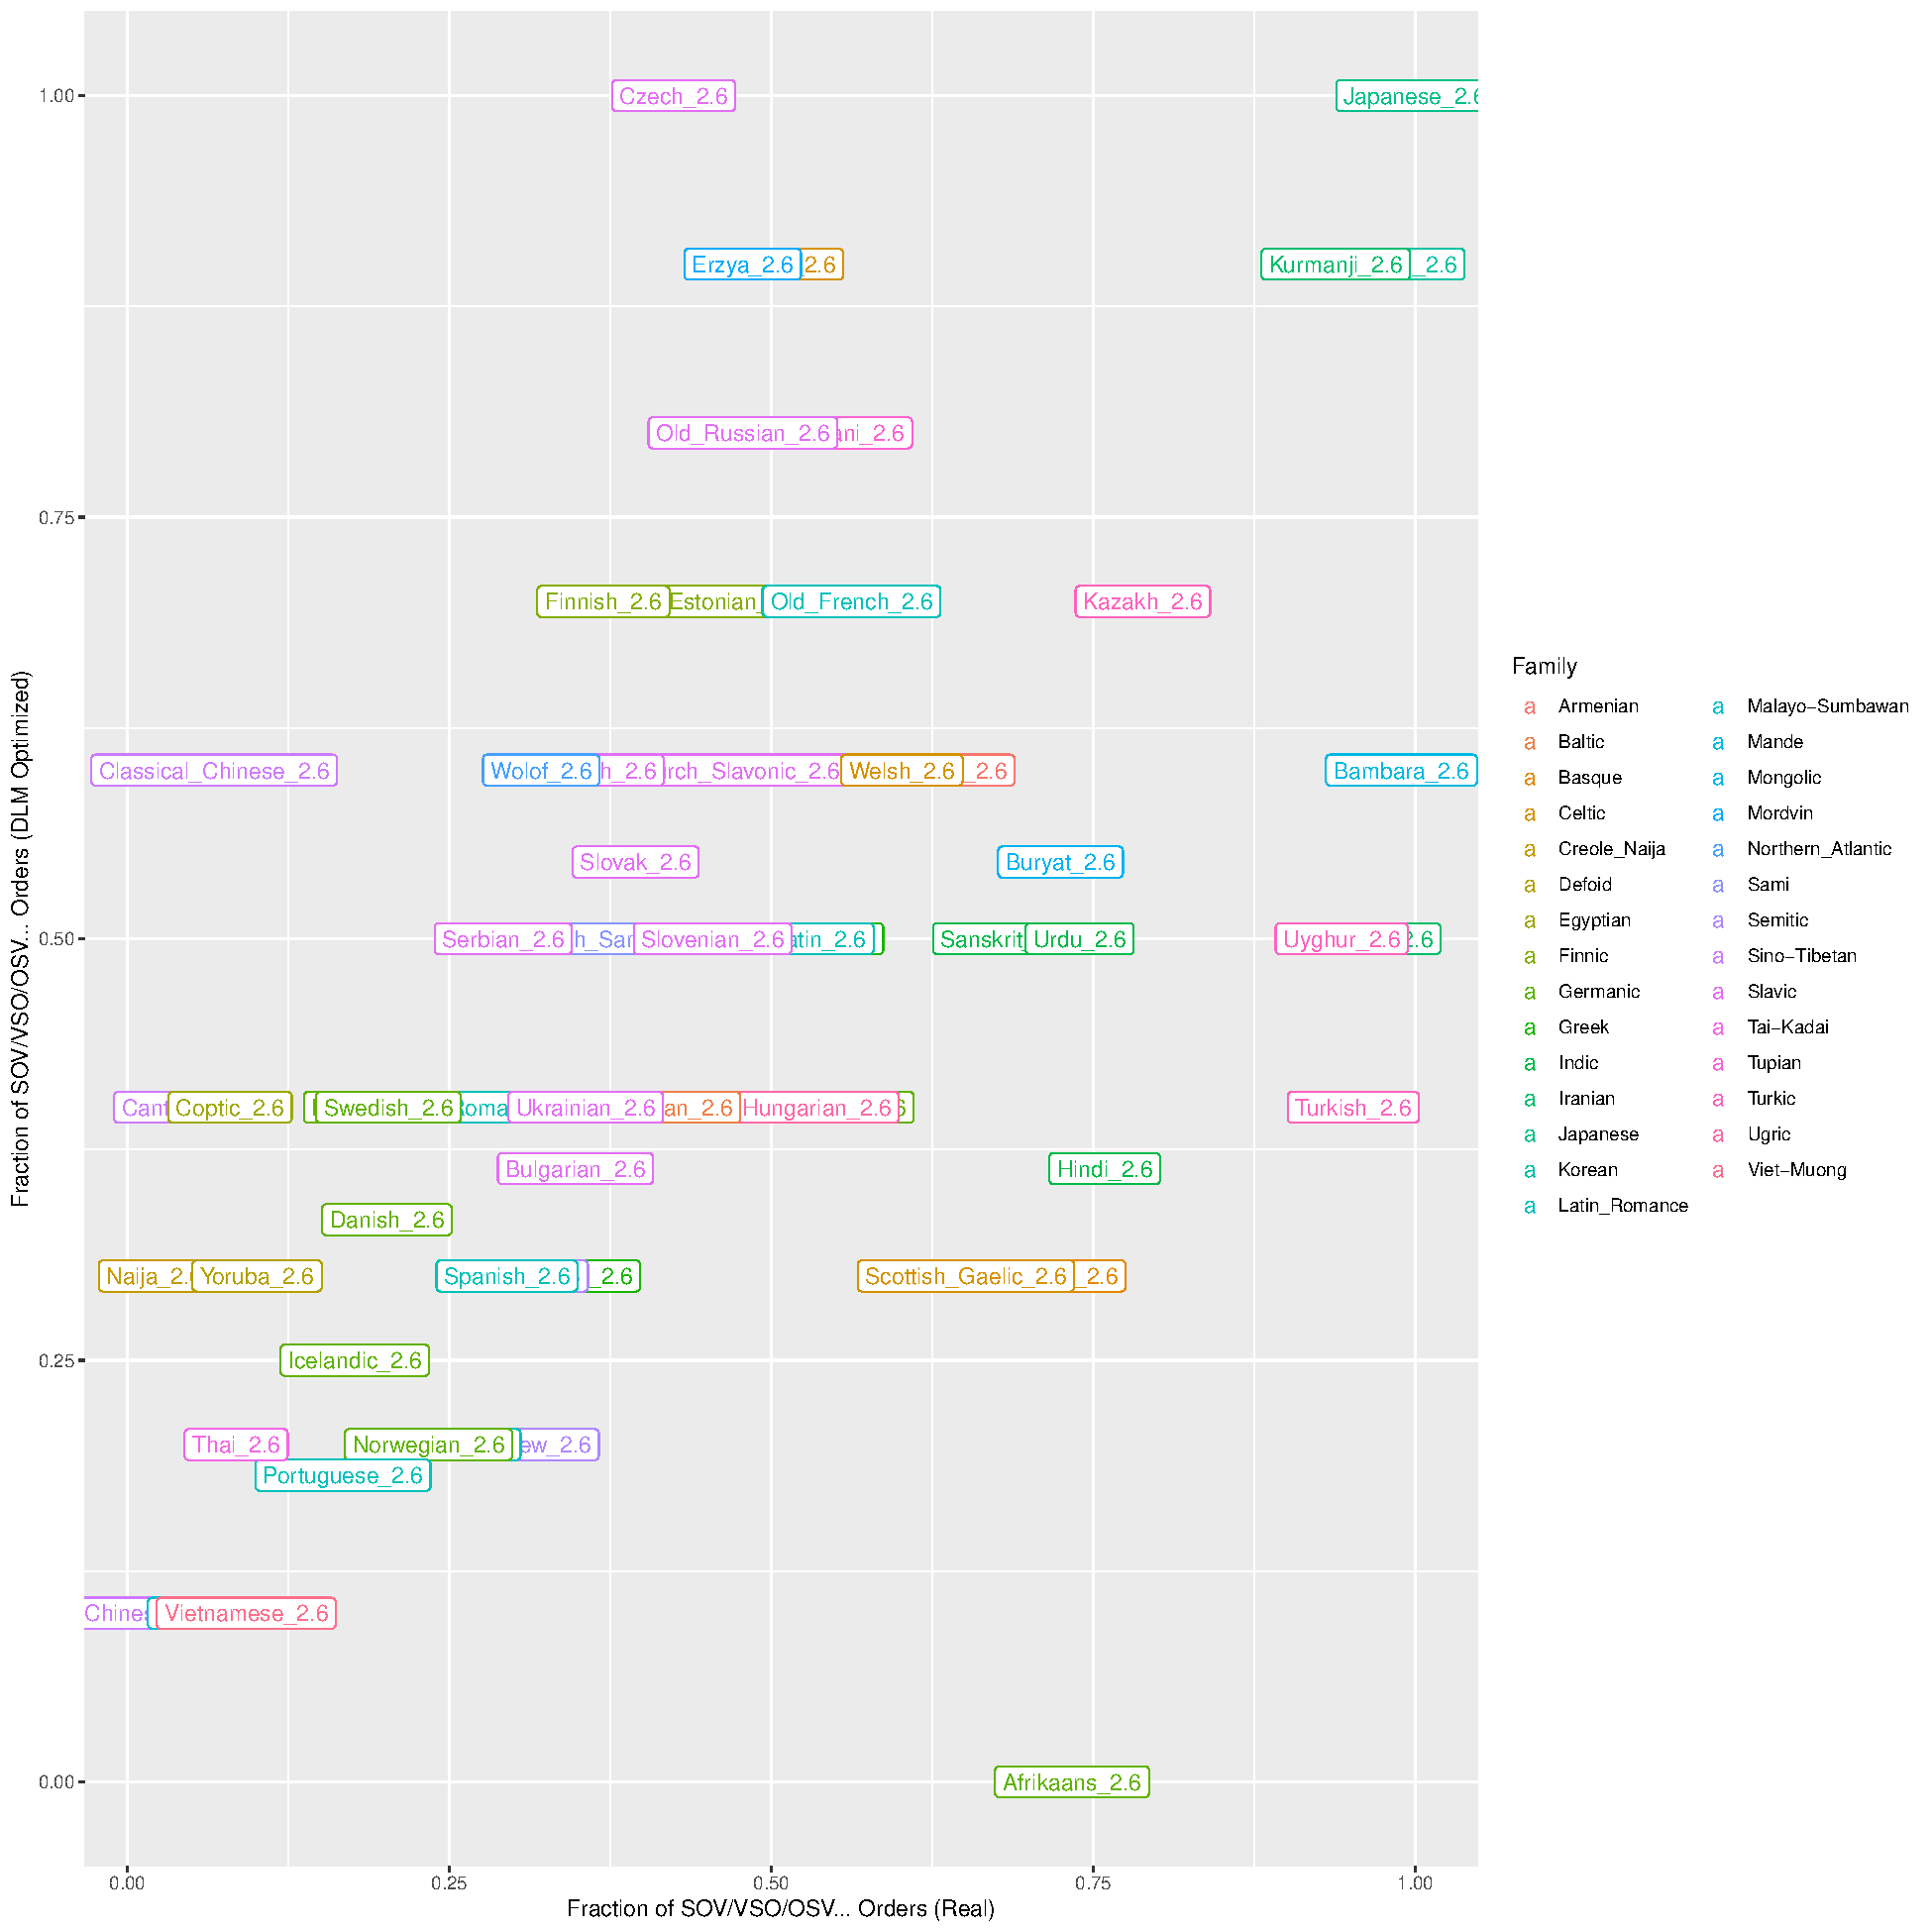
\includegraphics[width=0.7\textwidth]{figures/fracion-optimized_DLM_2.6.pdf}
    \caption{Study 1 (Prevalence of SOV-like order)}
    \label{fig:study1}
\end{figure}


\begin{figure}
    \centering
    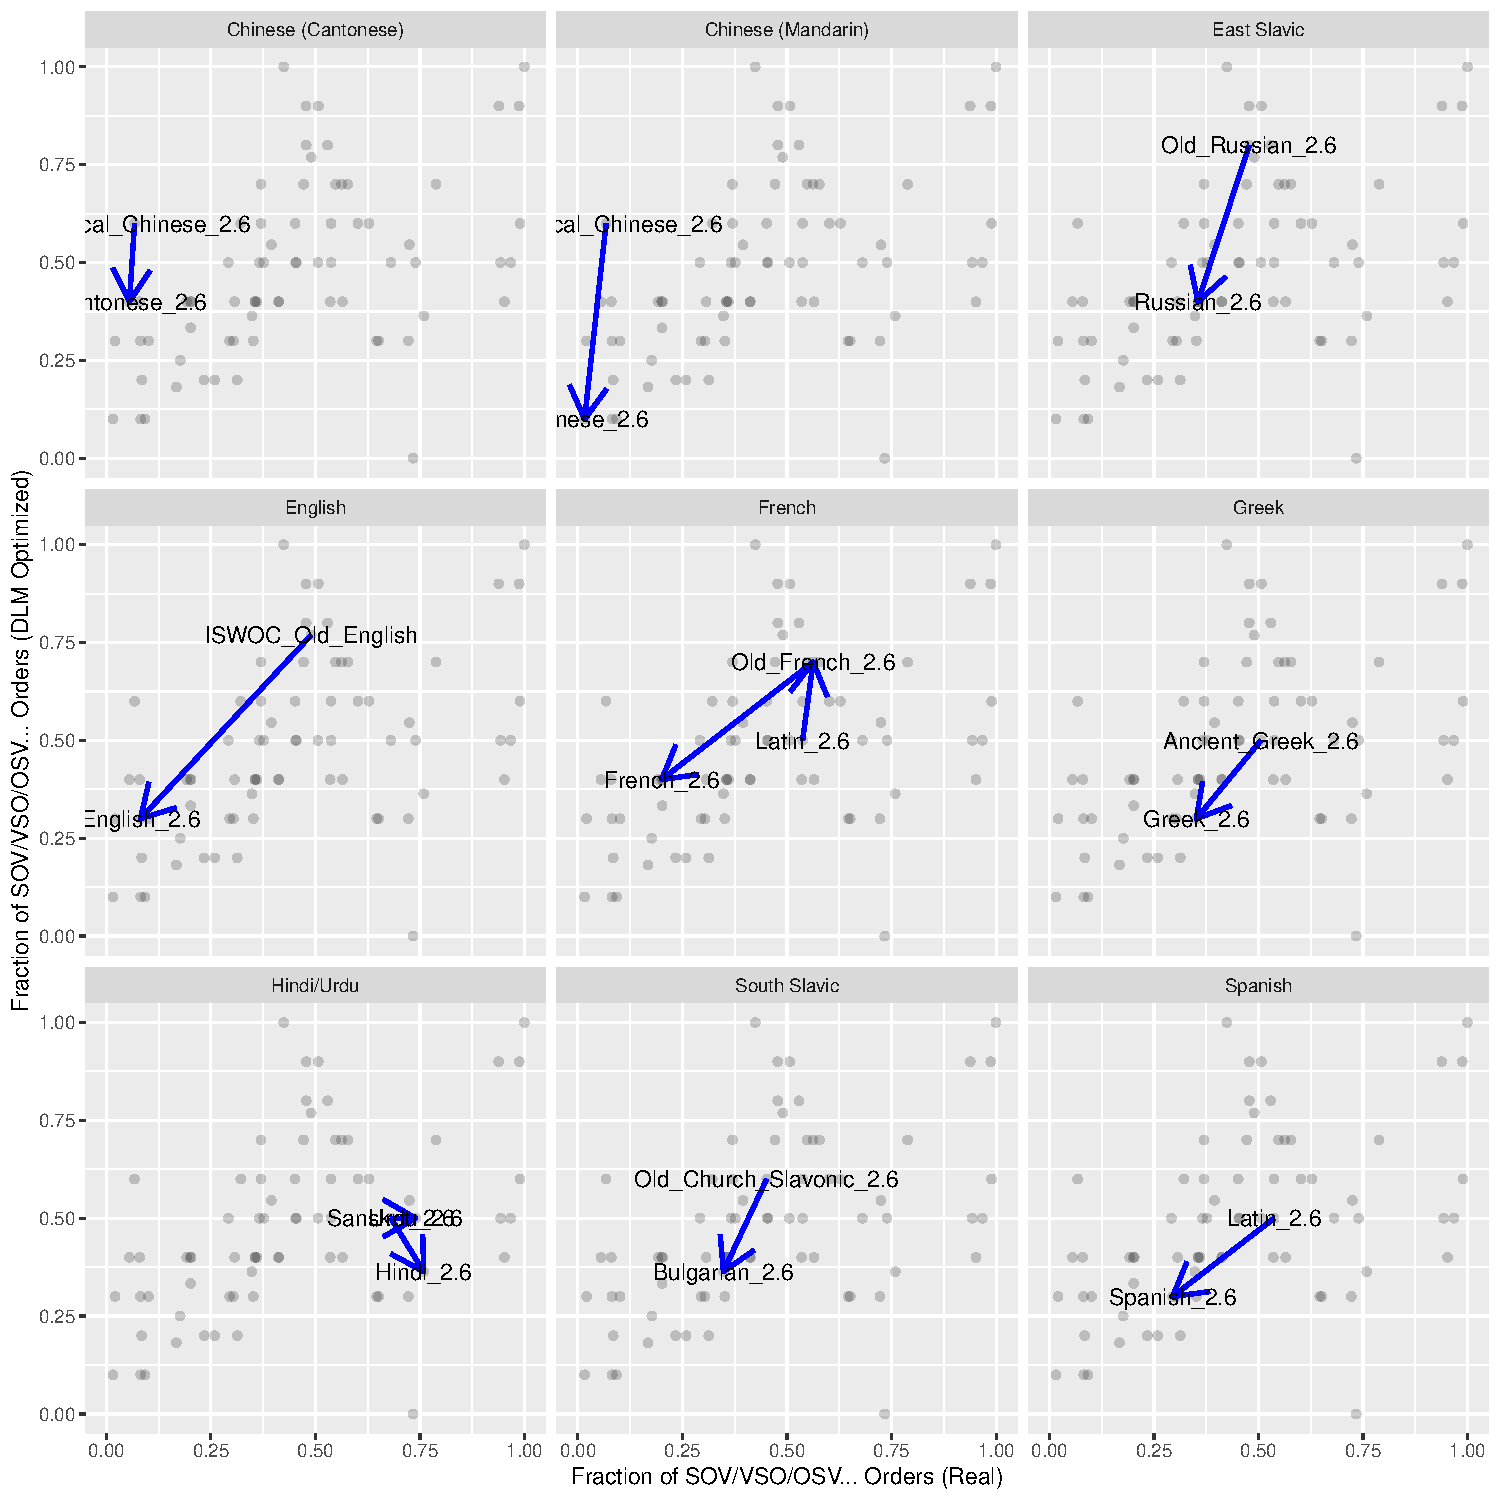
\includegraphics[width=0.7\textwidth]{historical_2.6.pdf}
    \caption{Study 1}
    \label{fig:study1}
\end{figure}




\section{Study 2: Co-Expressing Subjects and Objects}

-In what ways do usage patterns influence which word order is optimally efficient?

-Co-expression of subjects and objects (referenced from the thought experiment above)

-Results: Figure \ref{fig:study2} plus stats


\begin{figure}
    \centering
    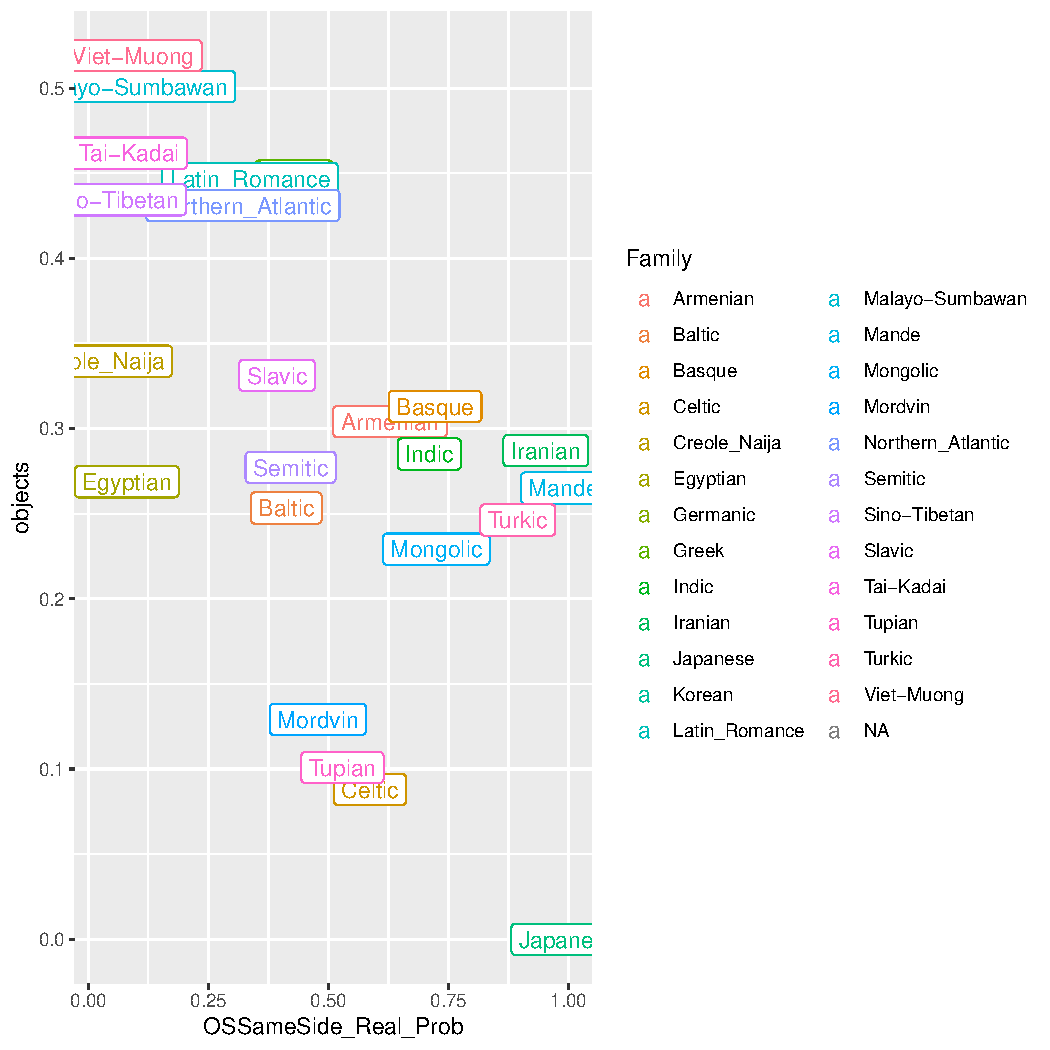
\includegraphics[width=0.7\textwidth]{figures/objects-order-families.pdf}
    \caption{Study 2 (Coexpression of suibjects and objects)}
    \label{fig:study2}
\end{figure}


%\section{Hypotheses}

%SVO preferred when S,O both present, and when O long and S short.

%SOV, VSO orders preferred when O short/not present/intransitive, and when embedded

%Relevant data

%- intransitive subjects behaving like objects

%- Continental West Germanic (except Yiddish). Main clauses predominant SVO/OSV; embedded clauses SOV/OSV.

%- languages with predominant VSO, but alternative SVO in matrix clauses: Standard Arabic, Berber, Ancient Egyptian

%- relative clauses in Bantu: Demuth,Katherine,andCarolynHarford.1999.Verb raising and subject inversion in Bantu relatives. Journal of African Languages and Lingustics20:41ñ61.


\section{Discussion}

\paragraph{Causal direction} can't decide. not logically necessary that there even is a single causal direction across languages and time.

\paragraph{Relation to prior work}

- our results argue against work that has suggested SVO as the more efficient order (Gibson et al 2013, \url{https://www.ncbi.nlm.nih.gov/pmc/articles/PMC4534792/})


\section{Conclusion}

\bibliography{literature}
\bibliographystyle{acl_natbib}


\end{document}



